\documentclass{article}
\usepackage{assumptionsofphysics}
\usepackage{graphicx}
\graphicspath{{images/}}
\usepackage{tikz}
\usetikzlibrary{shapes,backgrounds}
\usepackage{pgfplots}
\begin{document}
\title{DrawingFigs}

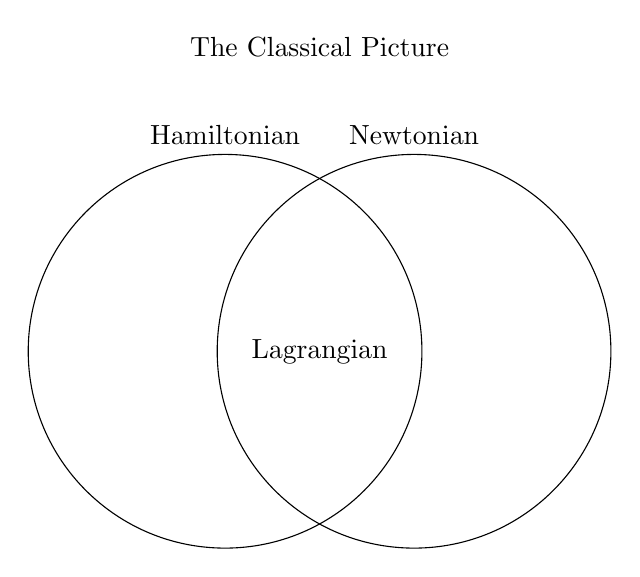
\begin{tikzpicture}
\title{Figure 1 Venn Diagram}

\node [label={The Classical Picture}] (C) at (1.2,3.5){};
 
% Set A
\node [draw,
    circle,
    minimum size =5cm,
    label={90:Hamiltonian}] (A) at (0,0){};
 
% Set B
\node [draw,
    circle,
    minimum size =5cm,
    label={90:Newtonian}] (B) at (2.4,0){};
 
% Set intersection label
\node at (1.2,0) {Lagrangian};
 
\end{tikzpicture}
\newpage

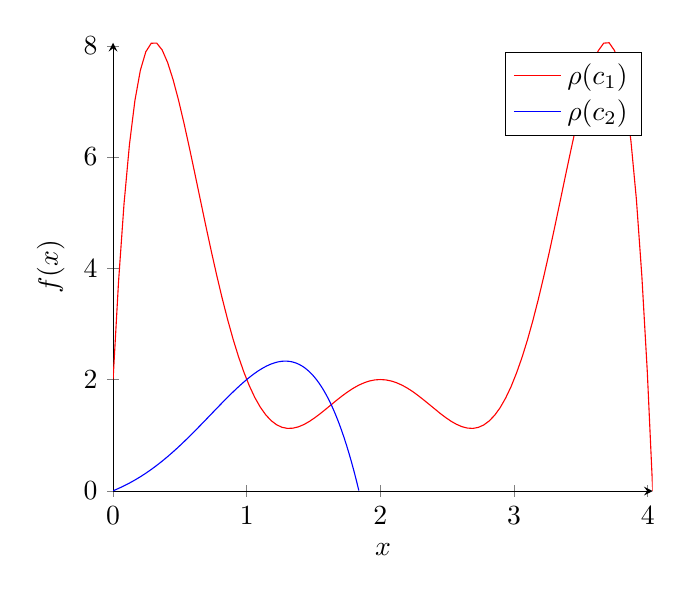
\begin{tikzpicture}
\title{C to S function}

\begin{axis}[
    axis lines = left,
    xlabel = \(x\),
    ylabel = {\(f(x)\)},
]
%Below the red parabola is defined
\addplot [
    domain=0:4.038, 
    samples=100, 
    color=red,
]
{-1*x^6+12*x^5-55*x^4+120*x^3-124*x^2+48*x+2};
\addlegendentry{\( \rho (c_1) \)}

\addplot [
    domain=0:1.839, 
    samples=100, 
    color=blue,
]
{-1*x^4+x+x^3+x^2};
\addlegendentry{\( \rho (c_2) \)}


\end{axis}
\end{tikzpicture}

\end{document}
